\subsection{Time of Flight Methods}

In a time of flight measurement the time $\Delta t=t_2-t_1$ is measured that an object needs to travel from one position $x_1$ to another position $x_2$. If the distance between the two positions $\Delta x=x_2-x_1$ is known, the mean velocity between the two positions is

\begin{equation}
v_{mean}=\frac{\Delta x}{\Delta t}.
\end{equation}

\subsection{The Compound Pendulum}

A compound pendulum consists of a rigid body with a moment of inertia $I$ that is swinging around a pivot. Its movement can be completely described by considering the angle $\varphi$ between the vector from the pivot to the center of mass $\vec{R}$ and the gravitational force $\vec{F}_g$ (in case a visualisation is needed see fig. \ref{fig:forces} in the following section). The force $\vec{F}_g$ exerts a back driving torque $\tau = (\vec{R} \times \vec{F_g})_z = -R F_g \sin \varphi$ on the body. For small angles $\varphi$ one can approximate $sin\varphi \approx \varphi$. Hence the angular equation of motion is

\begin{equation}
I\ddot{\varphi} = -R F_g \varphi.
\end{equation}
 
This is the equation for a simple harmonic oscillator with the angular frequency $\omega = \sqrt{\frac{R F_g}{I}}$ considering $F_g=Mg$ where $M$ is the mass of the body and $g$ is the gravitational constant. The solution to this equation is

\begin{equation}\label{eq:sho}
\varphi(t) = \varphi _0 \cos\left(\omega t + \delta\right).
\end{equation}

The assumption $\delta=0 \Rightarrow \varphi(t=0)=\varphi_0$ is made in the following discussion since the phase is not important in this context.

Now one can ask which energy is stored in such an oscillation. Assuming that at $\varphi=0$ the energy is only kinetic energy all the energy of the system at turning point $\varphi=\varphi_0$  should only consist of potential energy in the gravitational field. This potential energy is equal to the negative of the work that has to be performed \cite{torque} against the back driving torque $\tau$ if one moves the pendulum from the position  $\varphi=0$ to $\varphi=\varphi_0$ on get

\begin{equation}
W = \int_0^{\varphi_0} \tau(\varphi) d\varphi = -\int_0^{\varphi_0} R F_g \varphi d\varphi = -\frac{1}{2}
R F_g \varphi_0^2.
\end{equation}

So the relation between the energy of the oscillation $E=-W$ and its amplitude $\varphi_0$ is

\begin{equation}\label{eq:ephi}
\varphi_0 = \sqrt{\frac{2E}{R F_g}}.
\end{equation} 

This can now be plugged into eq. (\ref{eq:sho}). Due to the damping described in the following sections the amplitude will decay over time so that there is a time dependence $\varphi_0(t)$ and thus also the energy $E(t)$ will flow out of the system with time $t$. The assumption that the angular frequency $\omega$ stays constant during this process is empirically applicable for weakly damped oscillations; which gives that

\begin{equation}\label{eqphi}
\varphi(t) = \sqrt{\frac{2 E(t)}{R F_g}}  \cos\left(\omega t \right).
\end{equation}

If one differentiates this term it can be assumed that $E(t)$ varies much slower with time than $\cos\left(\omega t \right)$ which corresponds to the observation that $\varphi$ changes rapidly from $-\varphi_0$ to $+\varphi_0$ due to the oscillation with  $\omega$ whereas the decrease  $\varphi(t)>\varphi(t+T)$ is much smaller. So one can write that

\begin{equation}\label{eqphi_dot}
\dot{\varphi}(t) \approx  -\omega \sqrt{\frac{2 E(t)}{R F_g}} \sin\left(\omega t \right).
\end{equation}


\begin{figure}[h]
\begin{center}
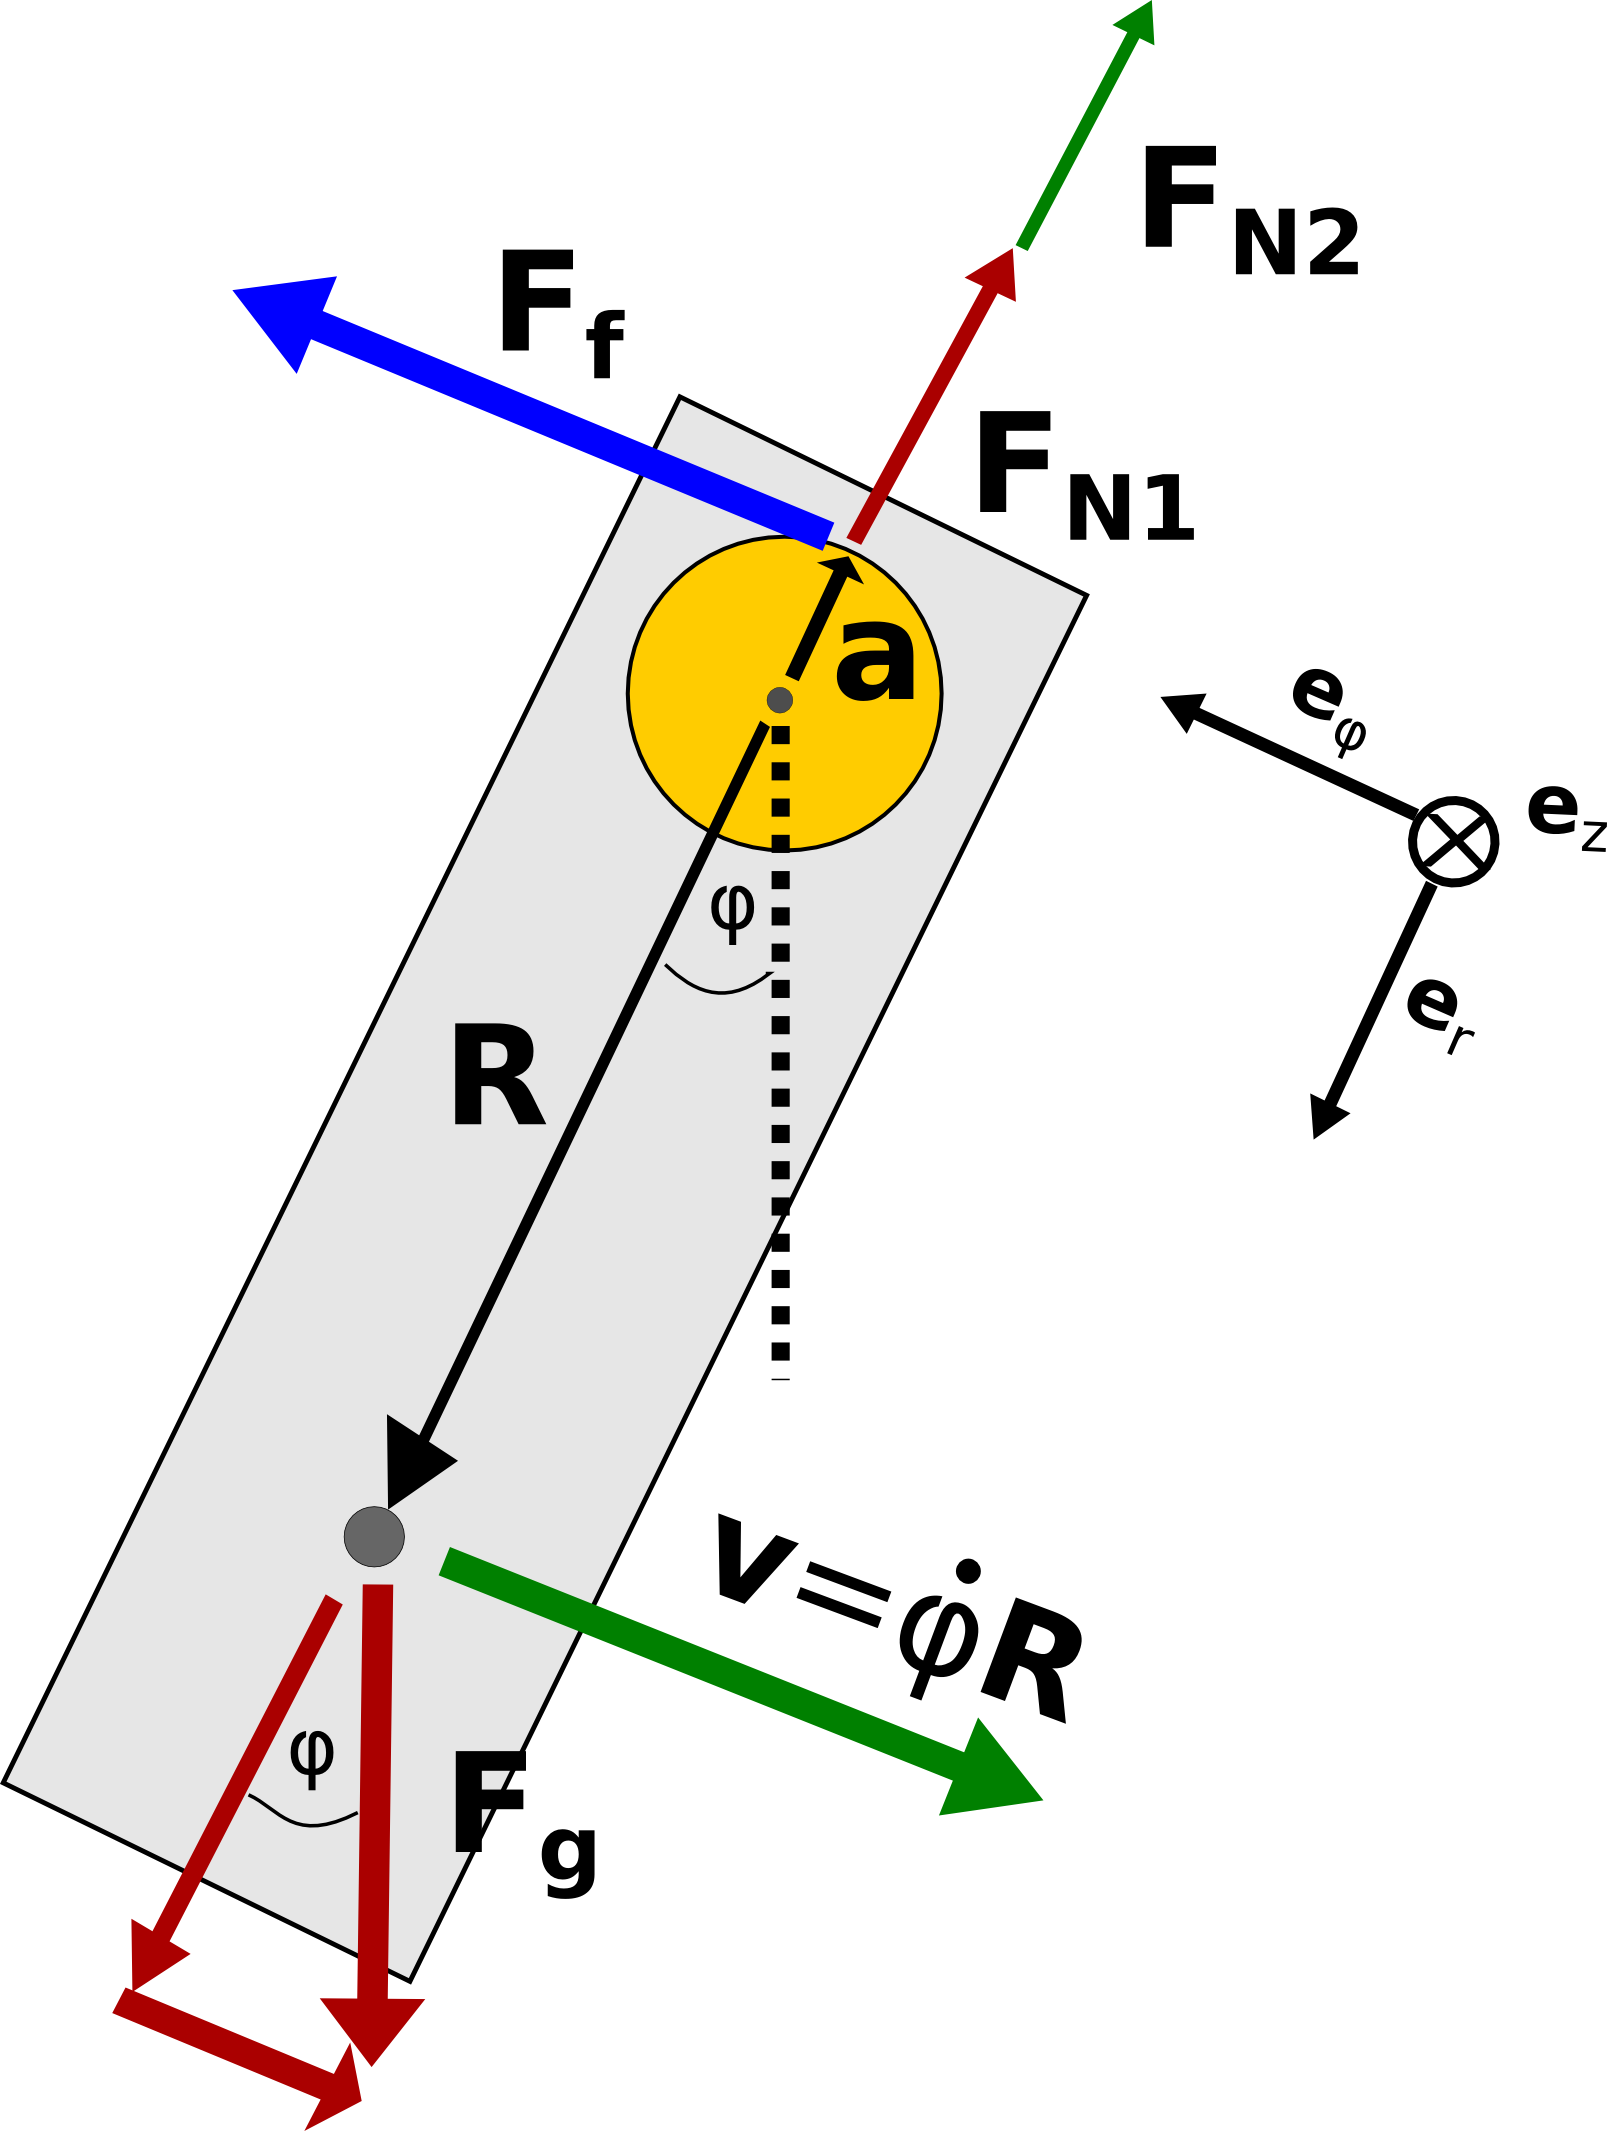
\includegraphics[scale=0.55]{img/forces.png}
\end{center}\caption{Geometry of the pendulum and forces acting during the oscillation with corresponding cylindrical coordinate system. (Vectors are bold)}\label{fig:forces}
\end{figure}


\subsection{The damping torque $\tau_f$ due to friction at the suspension point}

At the surface of the rod where the pendulum is suspended a friction force $F_f$ occurs during the oscillation. In Coulomb's model of friction \cite{friction} the friction force is considered as being proportional to the normal force $F_N$ that keeps the pendulum on its track. Since the pendulum is continuously moving, the proportionality constant is given by the coefficient of kinetic friction $\mu_k$ that depends on the used materials\footnote{Actually the pendulum stops in the turning points for a very short time. But as long as the coefficient of static friction $\mu_s$ is not much larger than $\mu_k$ this should not have a visible effect. For most materials $\mu_s$ and $\mu_k$ are in the same order of magnitude.}. So one gets the equation

\begin{equation}
F_f=\mu_k F_N.
\end{equation}

Regarding fig. \ref{fig:forces} it becomes clear that the normal force consists of two parts $F_N=F_{N1}+F_{N2}$ where:

\begin{itemize}
\item The force $F_{N1} = F_g \cos \varphi $  counters the component of the gravitational force that is acting in the direction of $\vec{R}$.
\item The force $F_{N2} = M \dot{\varphi}^2 R$  acts as a centripetal force to keep the pendulum on its circular path. \cite{centripetalforce}
\end{itemize}

If $a$ is the radius of the rod where the pendulum is fixed (see again figure \ref{fig:forces}), then the resulting torque due to the friction force is

\begin{equation}\label{eq:tauf}
\tau_f = a F_f = a \mu_k M \left(g \cos \varphi + \dot{\varphi}^2 R\right) \approx a \mu_k M \left(g - \frac{g}{2} \varphi^2  + \dot{\varphi}^2 R\right).
\end{equation}





\subsection{The damping torque $\tau_d$ due to the air drag}

Since the pendulum is moving quite fast and its shape is approximately circular so the air flowing around it should give rise to a lot of curls. In this case one can apply the drag equation \cite{airdrag} 
\begin{equation}\label{eq:coulomb}
F_d=\frac{1}{2} \rho v^2 C_D A.
\end{equation}

In this equation the following parameters occur:

\begin{itemize}
\item $\rho$ is the density of the fluid (here air).
\item $v$ is the velocity of the floating object.
\item $A$ is the cross-sectional area of the object.
\item $c_d$ is the \emph{air drag coefficient} that depends on the shape of the object.
\end{itemize}

However, this equation cannot be applied directly to the pendulum since each infinitesimal cross-sectional area element $dA=drdz$, see fig. \ref{fig:forces}, of it moves with a different velocity $v = \dot{\varphi}r$ depending on the distance $r$ from the pivot. So the infinitesimal force acting on $dA$ is given by $dF_d = \frac{1}{2} \rho  C_d  \dot{\phi}^2   r^2 dr dz$. It gives rise to an infinitesimal torque $d\tau = r dF_d$. 


If $L$ is the length of the pendulum ($\neq R$) and $d$ is its width the total torque due to the drag force is

\begin{equation}\label{eq:taug}
\tau_d = \int d\tau_d =  \frac{1}{2} \rho \dot{\phi}^2 C_d \int_0^L r^3 dr \int_0^d dz = \frac{1}{8}  \rho \dot{\varphi}^2  C_d L^4 d.
\end{equation}

\subsection{Determining the Time dependence of Energy $E(t)$}

Due to the frictional torques $\tau_D$ and $\tau_f$ derived in the sections above (eq. (\ref{eq:tauf}) and (\ref{eq:taug})) the energy of the oscillating System decreases. The ratio of this decrease $dE/dt$ is equal to the power $P=\left( \tau_D + \tau_f \right) \dot{\varphi}$ that the torques take out of the system. 
At this point it is crucial to consider that the equations \ref{eq:tauf} and \ref{eq:taug} only contain information about the absolute value of the torques. Since these torques describe friction, they should always act against the direction of $\dot{\varphi}$. So one has to add this information to get the correct result

\begin{equation}
P=-\rm{sign}\left(\dot{\varphi}\right) \left( \tau_D + \tau_f \right) \dot{\varphi} = -\left( \tau_D + \tau_f \right) \left|\dot{\varphi}\right|.
\end{equation} 

Now one can plug in $\tau_D$ and  $\tau_f$ respectively. One gets the differential equation

\begin{equation}
\frac{dE}{dt} = - \left( \frac{1}{8}  \rho \dot{\varphi}^2  C_D L^4 d + a \mu_k M \left(g - \frac{g}{2} \varphi^2  + \dot{\varphi}^2 R\right) \right)\left|\dot{\varphi}\right|.
\end{equation}

Defining the constants 
\begin{align}
A_1 &= \omega^3 \left(\frac{2}{R F_g}\right)^{3/2} \left(\frac{1}{8}  \rho  C_D L^4d+a \mu_k M R\right) \nonumber \\
A_2 &= \omega \left(\frac{2}{R F_g}\right)^{3/2}a \mu_k M \frac{g}{2} \nonumber \\
A_3 &= \omega \left(\frac{2}{R F_g}\right)^{1/2} a \mu_k M g \nonumber
\end{align}
 and plugging in eq. (\ref{eqphi_dot}) and (\ref{eqphi}) one gets

\begin{equation} \label{eq:full}
\frac{dE}{dt} = - A_1 E^\frac{3}{2} \left|\cos^3(\omega t)\right| - A_2 E^\frac{3}{2} \left|\cos(\omega t)\right|\sin^2(\omega t) - A_3 E^\frac{1}{2} \left|\cos(\omega t)\right|.
\end{equation}

This equation cannot be solved analytically but the program Mathematica can solve it numerically. In fig. \ref{fig:math} the result is visible. The right graph was calculated with with a higher angular frequency omega than the left one. 


\begin{figure}[h]
\begin{center}
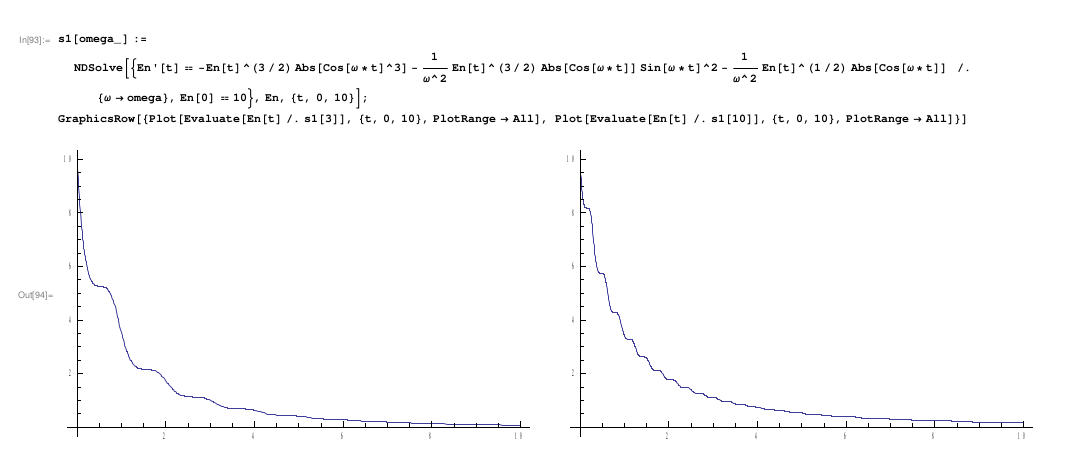
\includegraphics[scale=0.5]{img/results.png}
\end{center}\caption{Equation \ref{eq:full} solved numerically by Mathematica for two different values of $\omega$.}\label{fig:math}
\end{figure}

One can observe that the irregularities seem to vanish with a higher value for $\omega$. This is understandable from the fact that oscillations with high frequency do only produce very small fluctuations in the solution that are not visible. To get the solution without fluctuations one could take the mean value over time $<\left|\cos(\omega t)\right|> = <\left|\sin(\omega t)\right|> = \frac{1}{2}$. Defining new constants $B_1=\frac{1}{8}\left(A_1+A_2\right)$ and $B_2=\frac{1}{2}A_3$; then eq. (\ref{eq:full}) becomes

\begin{equation} \label{eq:fullshort}
\frac{dE}{dt} = - B_1 E^\frac{3}{2}  - B_2 E^\frac{1}{2}
\end{equation}

and have the analytical solution

\begin{equation}
E(t) = \frac{B_2}{B_1}\tan^2\left(\frac{\sqrt{B_1 B_2}}{2}t+C\right).
\end{equation}

This analytical function can be used later to fit the measured values. 

In case that the damping due to air drag is much bigger than the damping due to friction we can assume that $B_1 \gg B_2$. So eq. (\ref{eq:fullshort}) simplifies to

\begin{equation}
\frac{dE}{dt} = - B_1 E^\frac{3}{2}
\end{equation}


and has the solution

\begin{equation}\label{eq:air}
E(t)=\frac{4}{\left(B_1 t + C\right)^2}.
\end{equation}

%
%\begin{table}[htbp]
%	\centering
%		\begin{tabular}{l|c|c}
%		 $f$ [Hz] (detected)	 &  n			& prediction $f_n$  \\
%			\hline
%			75 & 1 & 85.4 \\
%			170 & 2    		& 170.75 \\
%			270 & 3 		& 256.1 \\
%			341  & 4 & (main) \\
%			450 & 5 & 426.9 \\
%			680  & 8 & 683  \\
%			880  & 10 & 853.8\\
%			1010 & 12 & 1024.5
%		\end{tabular}
%	\caption{Detected frequencies in comparison with the prediction $f_n=\frac{n}{4}f$}
%	\label{tab:density}
%\end{table}